\chapter{Solution}
\label{cha:solutioni}

%Give a (detailed) description of the approach:

%\begin{itemize}
%\item give reasons, why you decided for specific parts of the approach
%\item its also a good idea to compare with related work (because this
%		  approach did not work so well in \cite{conf/vldb/KenscheQXlYl07} the authors used..)
%\item In the proposal: a rough design (e.g., an architecture, algorithm) of the approach,
%		  clarifying what will be done by you and what is already there/is a ready-to-use part
%		  (e.g., a library, product you use). Give also some details about the technologies
%		  which you want to use in the thesis project.
%\item In the thesis: a conceptual description of your approach. Important: do not go into
%      implementation details at this stage. Give an overall picture (e.g., system architecture, data flow
%      diagram, sequence diagrams for an algorithm, etc.). Explain the main components of your solution
%      and give short description of any external or existing component which is used by your system.
%      Give conceptual models (e.g., EER diagrams) of your data structures.
%\item Important: describe the \emph{process} of getting to the final solution, do
%      not describe only the final solution. All design decisions are important (I preferred
%      X, because Y performs badly).
% \end{itemize}
At present due to the increment of mobile devices huge number of streaming data are being generated. Unfortunately, these datasets are not in an organised as it should be for the analysis. There are many null values in the dataset and the data are being high-dimensional as well. To analyse this kind of data we need to implement fast pre-processing steps to analyse those data sets. One of the important preprocessing technique is dimensionality reduction. 

An extensible framework to reduce the dimensions of streaming data with a concept of modularity of each component. To achieve this goal, framework is designed in such a way that each component act as a stand alone component but can be interacted with each other in a very convenient way. Moreover, the components are  plug-in and play designed architecture. Each component can be easily replaced or added more functionality through out the whole implementation phase when it is necessary.

In a broadshell, there are three modules of the whole framework which are listed below:
\begin{itemize}
	\item Data Set Load and Processing Module
	\item Dimensionality Reduction Module
	\item Visualization Module
\end{itemize}

Each module has its own responsibilty of the total framework. The task is divided in such a way so that the separation of concern principle exists. Each module is considered as a distinct section so that each section addresses a totally separate task. However, there are some interdependency of executing the order of component which will be addressed into the implementaiton part.

The architecture of the framework is the multitier architecture. From software engineering perspective in multitier architecture\footnote{\url{https://en.wikipedia.org/wiki/Multitier_architecture}} client-server are involved where presentation, application processing and data management functions are physically separated.
\begin{enumerate}
	\item Persistence Layer
	\item Business Layer
	\item Access Layer
	\item Presentation Layer
\end{enumerate}

According to the defintion from software perspective,  operation with the all data 

\begin{figure}[htbp]
	% center the image.
	\centering
	
	% include a png file. Adapt size to 0.5 * textwidth and retain aspect ratio (!)
	\resizebox{\textwidth}{!}{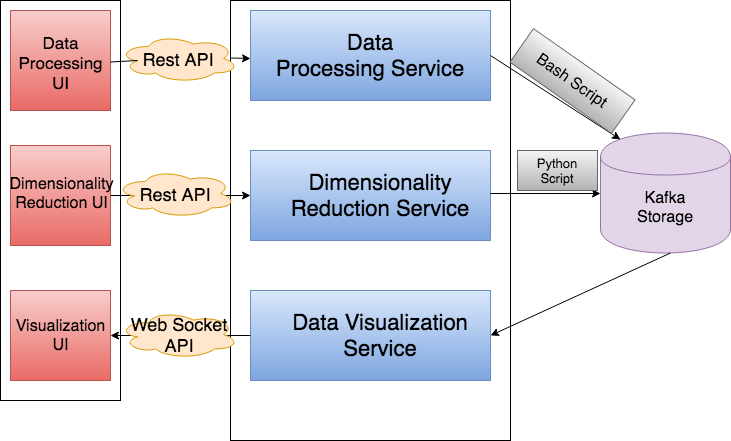
\includegraphics{architecture_thesisReport.png}}
	
	\caption{Architecture/ Design for the Extensible Framework}
	\label{fig:labelOfThesisFlowChart}
\end{figure}

In this section, I will describe the solution approach of reducing the high dimensional streaming data to low dimensional streaming data.\\\\
The following figure \ref{fig:labelOfThesisFlowChart} contains the general process model of our Framework.
\begin{figure}[htbp]
	% center the image.
	\centering
	
	% include a png file. Adapt size to 0.5 * textwidth and retain aspect ratio (!)
	\resizebox{\textwidth}{!}{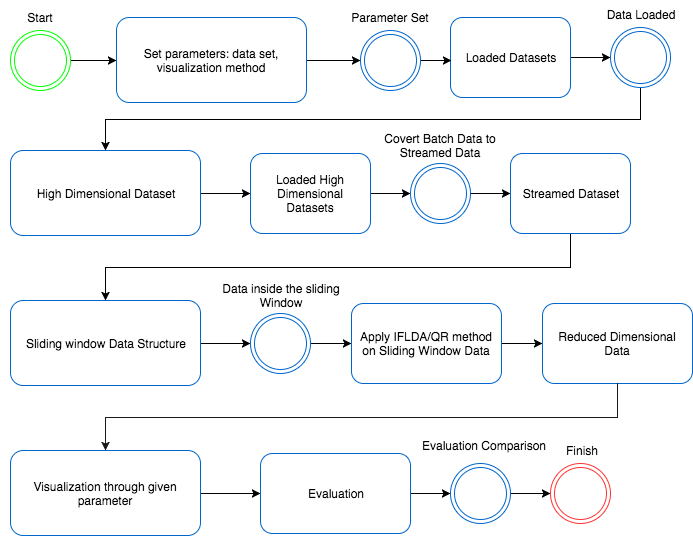
\includegraphics{Thesis_Flow_chart.png}}
	
	\caption{Dimensionality Reduction Framework of Streamed Data}
	\label{fig:labelOfThesisFlowChart}
\end{figure}
\subsection{Selection of Data Sets}
The framework will be flexible for both the online available streaming API to consider as a data source and also have the ability to upload the static data. Hence we are considering the streaming data it will be good if the chosen data domain have some impacts on the change of the data with the passage of the time.\\\\
If the chosen data set is not the streaming data then the framework will be capable enough to convert the static data to the streaming data using any available free state-on-art tools.
\subsection{Define Data Model}
The main characteristics of the streaming data that the data comes continuously with an unbounded structure and pattern as time progresses. For this reason, to handle the streaming data there should be some mechanism to hold the data for a minimum period of time and within that time all necessary work related with the data should be done then the data is thrown off. One of the common mechanism to handle those data is known as sliding window approach. Here the window is defined based on the time like in particular interval for example in each 500 ms the data comes are considered one window. The window will be moved after each fixed period of time and that's the reason it is known as sliding window approach. Our framework will be capable of considering the streaming data in a sliding window basis.
\subsection{IFLDA/QR algorithm}
As previously mentioned we will implement the IFLDA/QR algorithm. At the first window, we will implement the FLDA algorithm to calculate the centroid matrix and implement the Cholesky Decomposition of the centroid matrix. The output of this mechanism is the optimal transformation matrix.\\\\
From second window and so on we will implement the algorithm of the insertion of the chunk data. Here as an input of the process we will consider labeled new samples and also the novel class. Here the centroid matrix for an existing class will be updated as well as the new centroid of the new cluster will be calculated.In following figure \ref{fig:labelOfChunkData} the whole process is shown step by step wise.
\begin{figure}[htbp]
	% center the image.
	\centering
	
	% include a png file. Adapt size to 0.5 * textwidth and retain aspect ratio (!)
	\resizebox{\textwidth}{!}{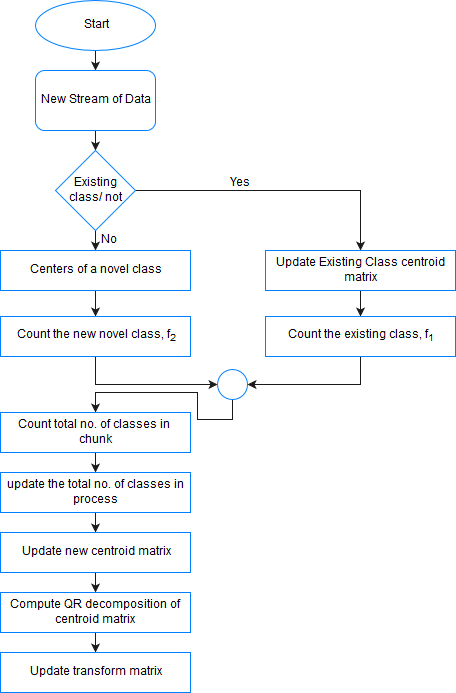
\includegraphics{chunk_data_process.png}}
	
	\caption{Process of Handling Stream Data}
	\label{fig:labelOfChunkData}
\end{figure}
\subsection{Data Visualization}
The final outcome of the framework will be the visualization. In visualization, we will see the inner relationship of the data. In this case, visualization will not be only used for the communication to the end user but also it will reveal the inner meanings of the data for example, the pattern of the data, the relationship among the features and many more. The visulaisation tool we used here will be the Heatmap, one of the most used visualization tool for high dimensional data.

\subsection{Design Framework}
In this section, we will describe the design of the framework in details. The framework should have ability to  extend for further implementation if needed. Moreover, the component should be reusable. The framework will also have the separation of concerns by allocating tasks to different layers.\\\\
The whole design Framework has four layers: 
\begin{enumerate}
	\item Persistence Layer
	\item Business Layer
	\item Access Layer
	\item Presentation Layer
\end{enumerate}
Each layer will be associated individual category of tasks. In Persistence layer the data will be saved and used for the tasks involved with data. The Business layer is responsible for doing all back end task for the framework. Through Access layer, Business layer and Presentation layer will communicate with each other where Presentation layer is responsible to present the data and take input from the user.\\\\   
This whole section will be further divided into three subsections. We will describe the requirements list at the beginning then the overall design of the framework and last but not the least the sequence diagram of the framework.
\subsubsection{List of Requirements }
The whole requirements for the framework will be described in this section. The framework should be adaptable enough to response based on the user input. Till now, the framework should meet the following requirements. 
\begin{enumerate}
	\item User can select data type from stream data or batch Data
	\item User can choose data set from available dataset
	\item User can add new dataset to the specified place by uploading to the framework
	\item User will get the reduced dimensional data for given input data
	\item User can select the time interval for observing the visualization
	\item User can select the required evaluation criteria from the evaluation list and show the evaluation information.
\end{enumerate}
\subsubsection{Architecture Diagram} 
In this section we will present the architecture diagram of the framework.  As mentioned, the architecture is divided into four sections and each section has separate components for the different concerns. In fig \ref{fig:labelOfFrameworkArchitecture}, each section is defined with the individual components. Each component is responsible for fixed set of requirements. Each layer has a bi-directional communication where one layer is communicated with others.
\begin{figure}[htbp]
	% center the image.
	\centering
	
	% include a png file. Adapt size to 0.5 * textwidth and retain aspect ratio (!)
	\resizebox{\textwidth}{!}{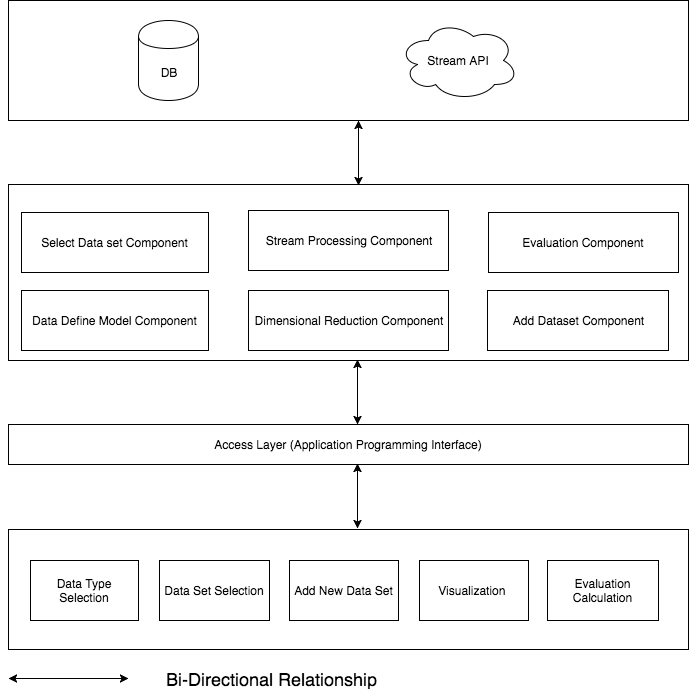
\includegraphics{DRFW_Visualization_Architecture.png}}
	
	\caption{Framework Architecture}
	\label{fig:labelOfFrameworkArchitecture}
\end{figure}
Based on the requirements a particular set of component is assigned for a fixed task. In Persistence layer, all information of the data is stored and ability to perform both read and write operation. There are in total five components in Business layer for performing all the requirements. The Access layer is all used for the communication using Application Programming Interface. There are five different ways for the user to communicate with the framework.
In Presentation layer, the user will send the parameter data to the Business layer \& receive data after the process done. In Business layer for implementing business logic it will communicate with the Persistence layer and send data to the front end. In addition, the business layer will also do the mathematical calculation for presenting evaluation information to the presentation layer. \\\\
In Presentation layer, user can give three inputs for showing the intended output: Select Data type, Dataset, Time interval selection, Select evaluation parameter. For adding new dataset user can upload to the framework. The details requirement list for the Presentaiton layer is listed below:
\begin{itemize}
	\item Select Data type: User can select either Stream Data or Batch Data
	\item Select Dataset: User can choose data set from Available Dataset
	\item Add new Dataset: User can add new dataset to the specified place by uploading
	\item Show Visualization based on given time interval: Here, user will select at what interval of time user wants to visualize and be able to watch visualization
	\item Evaluation Information: User can show the evaluation information for example information loss will be shown in continuous fashion
\end{itemize}
From Presentation layer the framework will access the Business layer through Access layer. The framework will have few Application Programming Interface associated with each task. In Business layer, the framework will implement the business logic of the framework. The details requirement list for the Business layer is listed below:
\begin{itemize}
	\item Save Datasets to Database: Framework should save the dataset that user gives to the Presentation layer and give feedback in both accept state or rejection state. The dataset should be available from that point on wards in the framework if accepted.
	\item List of available Datasets: If user selects the Batch data then framework should send all the  available datasets to the user for selection.
	\item Stream Processing: The framework should be able to detect whether selected type is batch or stream. If Selected type is stream than this component should not do any further tasks otherwise the framework will convert the static data to the stream data
	\item Data Define Model: After selection of the data the framework should capture the data for the fixed time window and apply the dimensionality reduction on that window.
	\item Dimensionality Reduction: Framework should be able to reduce the dimensions of the input dataset.
\end{itemize}

\subsubsection{Sequence Diagram}
In this section, the corresponding sequence of each requirement is described in details like how the request/ response is communicated from each layer through out the framework and also start or finishing time of any requirement. In fig \ref{fig:labelOfSequenceDiagram} the whole process is shown in details.
\begin{figure}[htbp]
	% center the image.
	\centering
	
	% include a png file. Adapt size to 0.5 * textwidth and retain aspect ratio (!)
	\resizebox{\textwidth}{!}{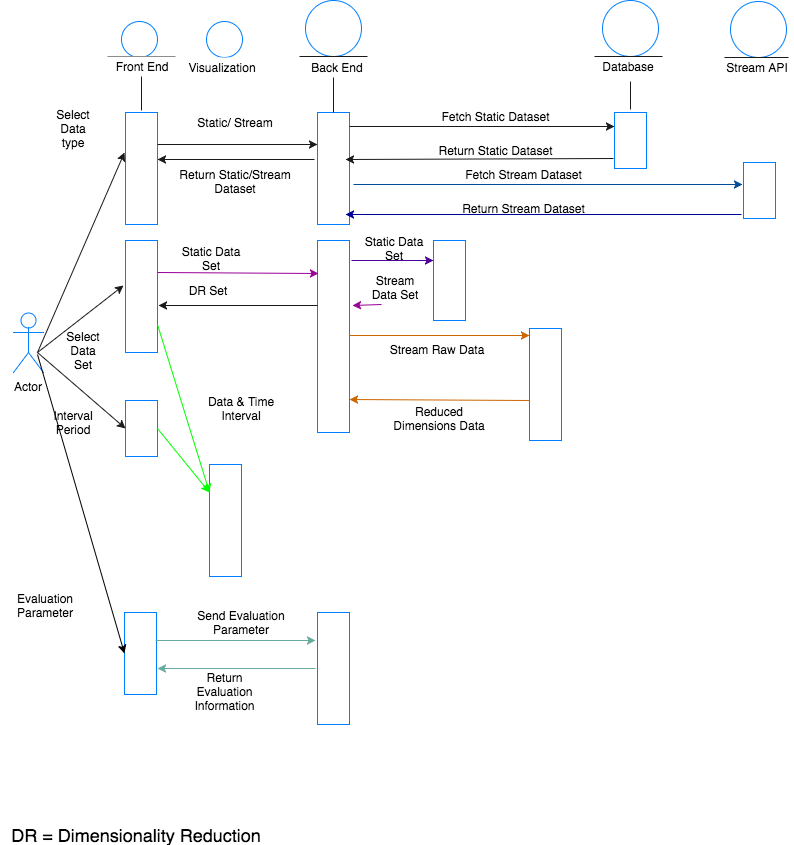
\includegraphics{Sequence_Diagram.png}}
	
	\caption{Sequence Diagram}
	\label{fig:labelOfSequenceDiagram}
\end{figure}
The total sequence diagram is explained in step wise one after another.
\paragraph{Selection of Data Type: }
User will select the data type and this value will be send to the backend. The value will be saved and send to "Select Data set" component . From backend, it will communicate to the database and receive the available data set. If the type is stream then it will directly communicate with the cloud and collect the available datasets from that stream. The dataset will be either a set of the static data or a set of streaming Application Program Interface.
\paragraph{Show Visualization based on time interval:}
User will select the time to define the frame of each window. This input will be required to the Business layer to "Data Define Model" component. User will also select time interval to see the visualization after a certain interval. For example, if the given interval value is 5 then user will see the visualisation after 5 window respectively.  
\paragraph{Selection of Data Set:}
User will select the data set from the available data set from the previous step . If the selected data set is "Batch" data set then from persistence layer it will go the "Stream Processing" component. The main task of this component is to convert static to stream data. If the type is "Stream" then this component has nothing to do other than sending void. This stream data will be used for further process.\\\\
Now the stream data along with the window frame size will go to the "Dimensional Reduction" component. This component is the heart of the framework. This component will be responsible to reduce the dimensions by implementing the algorithm and send back to Persistence layer. Based on the given interval value, the persistence layer will show the visualization in segment "Visualization" of the Persistence layer.
\paragraph{Evaluation Information:}
Here the list of all possible evaluation criteria will be given in "Evaluation" of the presentation layer. From the given value it will communicate with the "Evaluation" component of the persistence layer and show the value to the user.
\paragraph{Add new Dataset:}
User will also be able to add new data set or a cloud Stream API. From Presentation layer with the given data set it will go the Business layer. From there Business layer will communicate  with the Persistence layer and save the value. The datset or API should be available from that time on if required.

